\documentclass[a4paper]{article}

\title{Getting started with GumstixNXT and OpenEmbedded}
\author{David Brandt and Ulrik Pagh Schultz\\\{david.brandt,ups\}@mmmi.sdu.dk\\USD's Modular Robotics Lab\\University of Southern Denmark\\http://modular.mmmi.sdu.dk}
\date{\today}

\addtolength{\textwidth}{4cm}
\addtolength{\hoffset}{-2cm}

\usepackage[pdftex]{hyperref}
\usepackage{graphicx}

%\usepackage{courier}

\newcommand{\out}[1]{\texttt{#1}}
\newcommand{\promt}[1]{\texttt{\$ \textbf{#1}}}


\newcommand{~}{\~{}}


\begin{document} 

\maketitle

\subsection*{Version and changes}

Revision 1.3.1 (\today)
%
\begin{itemize}
\item From revision 1.2: added a bit of information on Ubuntu 10.04
  LTS, typographic fixes, spellcheck
\item From revision 1.1: fixed incorrect URLs, added information on
  terminal program, more complete explanation for GPIO setup.
\item From revision 1.0: updated required Ubuntu packages (g$++$, git-core)
\end{itemize}

\section{Introduction}
This document contains a very brief introduction to using embedded Linux on the gumstix overo boards. The document is based on various online sources, but mainly on information also available at www.gumstix.org. The hope is that this document will provide enough information to enable the reader to compile Linux for an Overo board and get it to boot, in this document only booting from a micro SD card will be discussed, however many more booting options are available.

This guide is assuming that the development host is running Ubuntu 10.04 LTS (all updates installed, see Appendix \ref{app:getting-linux} for a quick guide on getting Linux up and running), alternatively VMWare or VirtualBox can be used (see Appendix \ref{app:virtualized} for some notes on using a virtualized host). We will also assume that the reader has access to the serial console port on the overo board, for instance by using the Tobi expansion board or similar.

\section{Booting Linux}
First a short introduction to what is needed in order to boot Linux on an overo board.

In order to get Linux fully running a total of four elements are needed:
\begin{description}
\item[x-load] The first level bootloader, it is very small and simple and its purpose is to load the bigger and more advanced second level bootloader.
\item[u-boot] The second level bootloader, it is configurable to load many different kinds of operating systems in many different ways including network booting etc. 
\item[uImage] The actual Linux kernel, including drivers compiled into the kernel, but not loadable modules or programs.
\item[rootfs] The entire file system mounted at boot, including modules, libraries, home folders, utility programs etc.
\end{description}

So in order to get Linux up and running we need to build these four elements and transfer them to a SD card in a way that makes it possible to boot from that card.
%
Let us first consider the tools needed.

\section{Installing OpenEmbedded}
OpenEmbedded (OE) is a build system used for the overo boards to create Linux distributions. OE is used to build all the parts we need for our Linux distribution including cross compilers, the kernel, rootfs etc. First we will take a look at how to setup OE.

The heart of OE is the BitBake program and a collection of recipes used by bitbake. The recipes contains information on how to compile and build a given package, along with dependencies and URLs for where to get the source code. It is used to create both the cross compiler, the bootloaders, the kernel and the root file system.

In order for OE to work on Ubuntu 10.04 LTS you need to install a number of packages, this can be done simply by using apt-get. The needed packages are: 

\begin{quote}
git-core, subversion, gcc, patch, help2man, diffstat, texi2html, texinfo,
libncurses5-dev, cvs, gawk, python-dev, python-pysqlite2, unzip,
chrpath, ccache, g$++$
\end{quote}

\noindent The command to do this would e.g.\ be the following:

\promt{sudo apt-get install git-core subversion gcc patch help2man diffstat texi2html texinfo libncurses5-dev cvs gawk python-dev python-pysqlite2 unzip chrpath ccache g++}

If you are using Ubuntu then be aware that it is likely that /bin/sh is linked to /bin/dash. If this is the case you need to change it to be linked to /bin/bash. This can be done by executing the following command and answering 'no' when asked whether to install dash as /bin/bash:

\begin{quote}
\promt{sudo dpkg-reconfigure dash}
\end{quote}

After installing the needed packages we need to get hold of the OE source files. Be aware that some of the following steps can generate significant amounts of data traffic. Further, when compiling complete distributions a lot of computing time and hard drive space will be needed. It is recommended that you have at least 10GB of free space if you want to compile distributions containing many utility programs etc.\footnote{Make sure to use a native Linux file system (not networked or mounted via virtualization) and do not move the installation around after you have completed building.}

As a first step we will create a directory for OE which will be were we locate all the files needed and generated while we work, through out this document we will assume that this directory is located at the root of your home folder and is named 'overo-oe', however this is by no means mandatory.

\begin{quote}
\promt{mkdir -p ~/overo-oe}\\
\promt{cd ~/overo-oe}
\end{quote}

(Note: if you copy-paste these commands, make sure that the
``\verb+~+'' character is correctly transferred.)
Now we will install the OE data and check out the overo Linux branch (there might be some warnings from the git commands, you should just ignore those):

\begin{quote}
\promt{git clone git://gitorious.org/gumstix-oe/mainline.git org.openembedded.dev}\\
\promt{cd org.openembedded.dev}\\
\promt{git checkout --track -b overo origin/overo}
\end{quote}

Next we install BitBake:
\begin{quote}
\promt{cd ~/overo-oe}\\
%\promt{git clone git://git.openembedded.net/bitbake bitbake}\\
\promt{git clone git://github.com/openembedded/bitbake bitbake}\\
\promt{cd bitbake}\\
\promt{git checkout 1.10.2}
\end{quote}
%openembedded.net er nede, desuden b�r github give bedre performance

Now we will copy the gumstix profile script files to our build directory:
\begin{quote}
\promt{cd ~/overo-oe}\\
\promt{cp -r org.openembedded.dev/contrib/gumstix/build .}
\end{quote}

In order to setup the environment variables for the build system we need to modify the bash profile, this can be done by the following command (you might want to backup .bashrc before issuing it):

\begin{quote}
\promt{cat ~/overo-oe/build/profile >> ~/.bashrc}
\end{quote}

In order for the changes to take effect you need to close your
terminal window and open a new one.  (Alternatively, you can load the
profile file into your current environment using the command
\promt{source build/profile})

\section{Building Linux}
Now we are done installing OE and are getting ready to build our Linux image. In order to build our own custom distribution we need to create a \emph{recipe} which tells bitbake what to include in our distribution. First we create the directory which should contain our custom recipes:

\begin{quote}
\promt{cd ~/overo-oe}\\
\promt{mkdir -p user.collection/recipes/images}
\end{quote}

In the directory we just created you should put all recipes you make yourself, you are not supposed to modify the recipes provided as part of the OE installation. Now, in the new directory create a file named \emph{myimage.bb} containing the following:

\begin{quote}
\begin{verbatim}
IMAGE_PREPROCESS_COMMAND = "create_etc_timestamp"

IMAGE_INSTALL = "task-boot \
            util-linux-ng-mount util-linux-ng-umount \
            angstrom-version \
            "

export IMAGE_BASENAME = "minimalist-image"

inherit image
\end{verbatim}
\end{quote}
%            SPLASH \

This bitbake recipe will build a fairly small, but not minimal, Linux distribution. In order to build the distribution use the following command:

\begin{quote}
\promt{cd ~/overo-oe}\\
\promt{bitbake myimage}
\end{quote}
 
You should be aware that this command will potentially take a long time (on the order of hours, depending on available processing power and network bandwidth). Briefly stated this small script instructs bitbake to build a small root file system for our Linux distribution, however, since bitbake takes care of all dependencies for us, this might involve compiling and building the cross compiler to compile the programs in the root file system and the Linux kernel itself plus actually compiling the Linux kernel, the needed kernel modules and utility programs. Further, the source code for many of these steps might not be available locally so they have to be downloaded before compiling them. The process will create a directory named \emph{~/overo-oe/tmp/} do not delete or modify the contents of this directory, this is where the temporary files generated during the build and the actual result will be stored. By keeping the temporary files repeated builds will be much faster. 

Once the build is completed you can find the generated files in the \emph{~/overo-oe/tmp/deploy/glibc/images/overo} at this point it should contain the u-boot boot loader (\emph{u-boot-overo.bin}), the kernel image (\emph{uImage-overo.bin}) and the root file system (\emph{minimalist-image-overo.tar.bz2}) along with some other files. So we still need the first level boot loader. In order to generate this use the command:

\begin{quote}
\promt{cd ~/overo-oe}\\
\promt{bitbake x-load}
\end{quote}

This will create the file \emph{MLO-overo} in the \emph{~/overo-oe/tmp/deploy/glibc/images/overo} directory.

\section{Booting from an SD Card}

\subsection{Installing Linux on the board}

The gumstix boards comes with Linux preinstalled, however, I recommend using the SD card slot for booting the boards. The reason for this is that if the contents of the onboard flash memory gets corrupted due to an error during development it can be difficult to reflash, however, an SD Card can easily be replaced.

The gumstix overo boards are able to boot directly from a micro SD or SDHC card. The following instructions will guide you how to make an SD card bootable an how to install your bootloaders and Linux distribution on it.

In order to create the needed partition layout we will use \emph{fdisk} an during the guide I will assume that the SD card is referred to by the device name \emph{/dev/sde}, this might be different on your machine.

First we need to unmount the card in order to modify it using fdisk:

\begin{quote}
\promt{sudo umount /dev/sde1}
\end{quote}

Next we start fdisk, and start building a new partition table:
\begin{quote}
\promt{sudo fdisk /dev/sde}\\
\out{Command (m for help): \textbf{o}}\\
\out{Building a new DOS disklabel. Changes will remain in memory only, until you decide to write them. After that, of course, the previous content won't be recoverable.}\\
\out{Warning: invalid flag 0x0000 of partition table 4 will be corrected by w(rite)}
\end{quote}

First we need information about the size of the card we are using:
\begin{quote}
\out{Command (m for help): \textbf{p}}\\
\out{Disk /dev/sde: 2032 MB, 2032664576 bytes}\\
\out{64 heads, 63 sectors/track, 984 cylinders}\\
\out{Units = cylinders of 4032 * 512 = 2064384 bytes}\\
\out{Disk identifier: 0x00aa8e5c}\\
\out{Device Boot Start End Blocks Id System}
\end{quote}

This particular example is for a 2GB card. In order to boot properly we need the to have a card formatted with 255 heads, 63 sectors and as many cylinders as we can fit. To calculate the number of cylinders, take the number of bytes reported above by fdisk, divide by 255 heads, 63 sectors and 512 bytes per sector. In our example: 2032664576 / 255 / 63 / 512 = 247.12 which we round \textbf{down} to 247 cylinders.

In order to make these settings in fdisk we enter expert mode and return to normal mode after we are done:
\begin{quote}
\out{Command (m for help): \textbf{x}}\\
\out{Expert command (m for help): \textbf{h}}\\
\out{Number of heads (1-256, default 4): \textbf{255}}\\
\out{Expert command (m for help): \textbf{s}}\\
\out{Number of sectors (1-63, default 62): \textbf{63}}\\
\out{Warning: setting sector offset for DOS compatibility}\\
\out{Expert command (m for help): \textbf{c}}\\
\out{Number of cylinders (1-1048576, default 984): \textbf{247}}\\
\out{Expert command (m for help): \textbf{r}}
\end{quote}

The boot loaders and the kernel image must be placed in the first partition on the card, which must be a FAT partition. Next step is to create a 32MB FAT partition and mark it as bootable:
\begin{quote}
\out{Command (m for help): \textbf{n}}\\
\out{Command action}\\
\out{e   extended}\\
\out{p   primary partition (1-4)}\\
\out{\textbf{p}}\\
\out{Partition number (1-4): \textbf{1}}\\
\out{First cylinder (1-247, default 1): \textbf{1}}\\
\out{Last cylinder or +size or +sizeM or +sizeK (1-247, default 15): \textbf{+32M}}\\
\out{Command (m for help): \textbf{t}}\\
\out{Selected partition 1}\\
\out{Hex code (type L to list codes): \textbf{c}}\\
\out{Changed system type of partition 1 to c (W95 FAT32 (LBA))}\\
\out{Command (m for help): \textbf{a}}\\
\out{Partition number (1-4): \textbf{1}}
\end{quote}

Next we need to create an ext3 partition on the rest of the card for the root file system and write our changes to the card:
\begin{quote}
\out{Command (m for help): \textbf{n}}\\
\out{Command action}\\
\out{e   extended}\\
\out{p   primary partition (1-4)}\\
\out{\textbf{p}}\\
\out{Partition number (1-4): \textbf{2}}\\
\out{First cylinder (6-247, default 6): \textbf{6}}\\
\out{Last cylinder or +size or +sizeM or +sizeK (6-247, default 247): \textbf{247}}\\
\out{Command (m for help): \textbf{w}}\\
\out{The partition table has been altered!}\\
\out{Calling ioctl() to re-read partition table.}\\
\out{WARNING: If you have created or modified any DOS 6.x partitions, please see the fdisk manual page for additional information.}\\
\out{Syncing disks}\\
\end{quote}

Next we need to format the two new partitions. First the FAT partition and then the ext3 partition.
\begin{quote}
\promt{sudo mkfs.vfat -F 32 /dev/sde1 -n FAT}\\
\promt{sudo mkfs.ext3 /dev/sde2}
\end{quote}

Now the card is ready to be populated with our newly build Linux distribution. First we mount the FAT partition and copy the boot loaders and the kernel image to it. Note that the first level boot loader \textbf{must} be written first. Also note that while we copy the files we also rename them such that the have the names expected by the boot loaders.
\begin{quote}
\promt{sudo mount /dev/sde1 /media/card}\\
\promt{cd ~/overo-oe/tmp/deploy/glibc/images/overo}\\
\promt{sudo cp MLO-overo /media/card/MLO}\\
\promt{sudo cp u-boot-overo.bin /media/card/u-boot.bin}\\
\promt{sudo cp uImage-overo.bin /media/card/uImage}\\
\promt{sudo umount /dev/sde1}
\end{quote}

Now the card contains a bootable Linux kernel, however without a root file system it is not of much use. The final steps installs the root file system in the ext3 partition.
\begin{quote}
\promt{sudo mount /dev/sde2 /media/card}\\
\promt{cd /media/card}\\
\promt{sudo tar xvaf ~/overo-oe/tmp/deploy/glibc/images/overo/minimalist-image-overo.tar.bz2}\\
\promt{cd}\\
\promt{sudo umount /dev/sde2}
\end{quote}

Now you can insert the SD card into the card reader on the gumstix module and power it on, and hopefully it should boot. When booting you might see some error messages such as: \emph{uncorrectable error: end\_request: I/O error, dev mtdblock0, sector 0}. These can be ignored.

\subsection{Connecting to the board}

The board connects to your computer via the USB cable, communication
is done using a terminal program, this enables you to run a shell
directly on the board with input/output taking place via your
computer.

The recommended programs for communicating with the board are minicom
and putty.  They should be setup for no flow control, 115200 baud 1N8.
You can connect via /dev/ttyUSB$n$, where $n$ is the number assigned
by Linux whenever you connect the device (this might change from time
to time).
%
Using the terminal program, you can see the messages at boot time, 
login as ``root'' and execute commands interactively.

\section{Working with the device}

We are now ready to start interfacing to the hardware on the device.
For this to work, the hardware must be configured correctly at
boot-time and there must not be any conflicting use of hardware
resources.  We use GPIO to interface to the hardware; GPIO can be
accessed from user-level using a generic interface and using a
dedicated kernel module.  We use the generic interface for initial
experiments (this section) and the dedicated kernel module to
implement the driver (next section).

\subsection{Configuring u-boot port setup to enable LED access}

\begin{figure}
\begin{center}
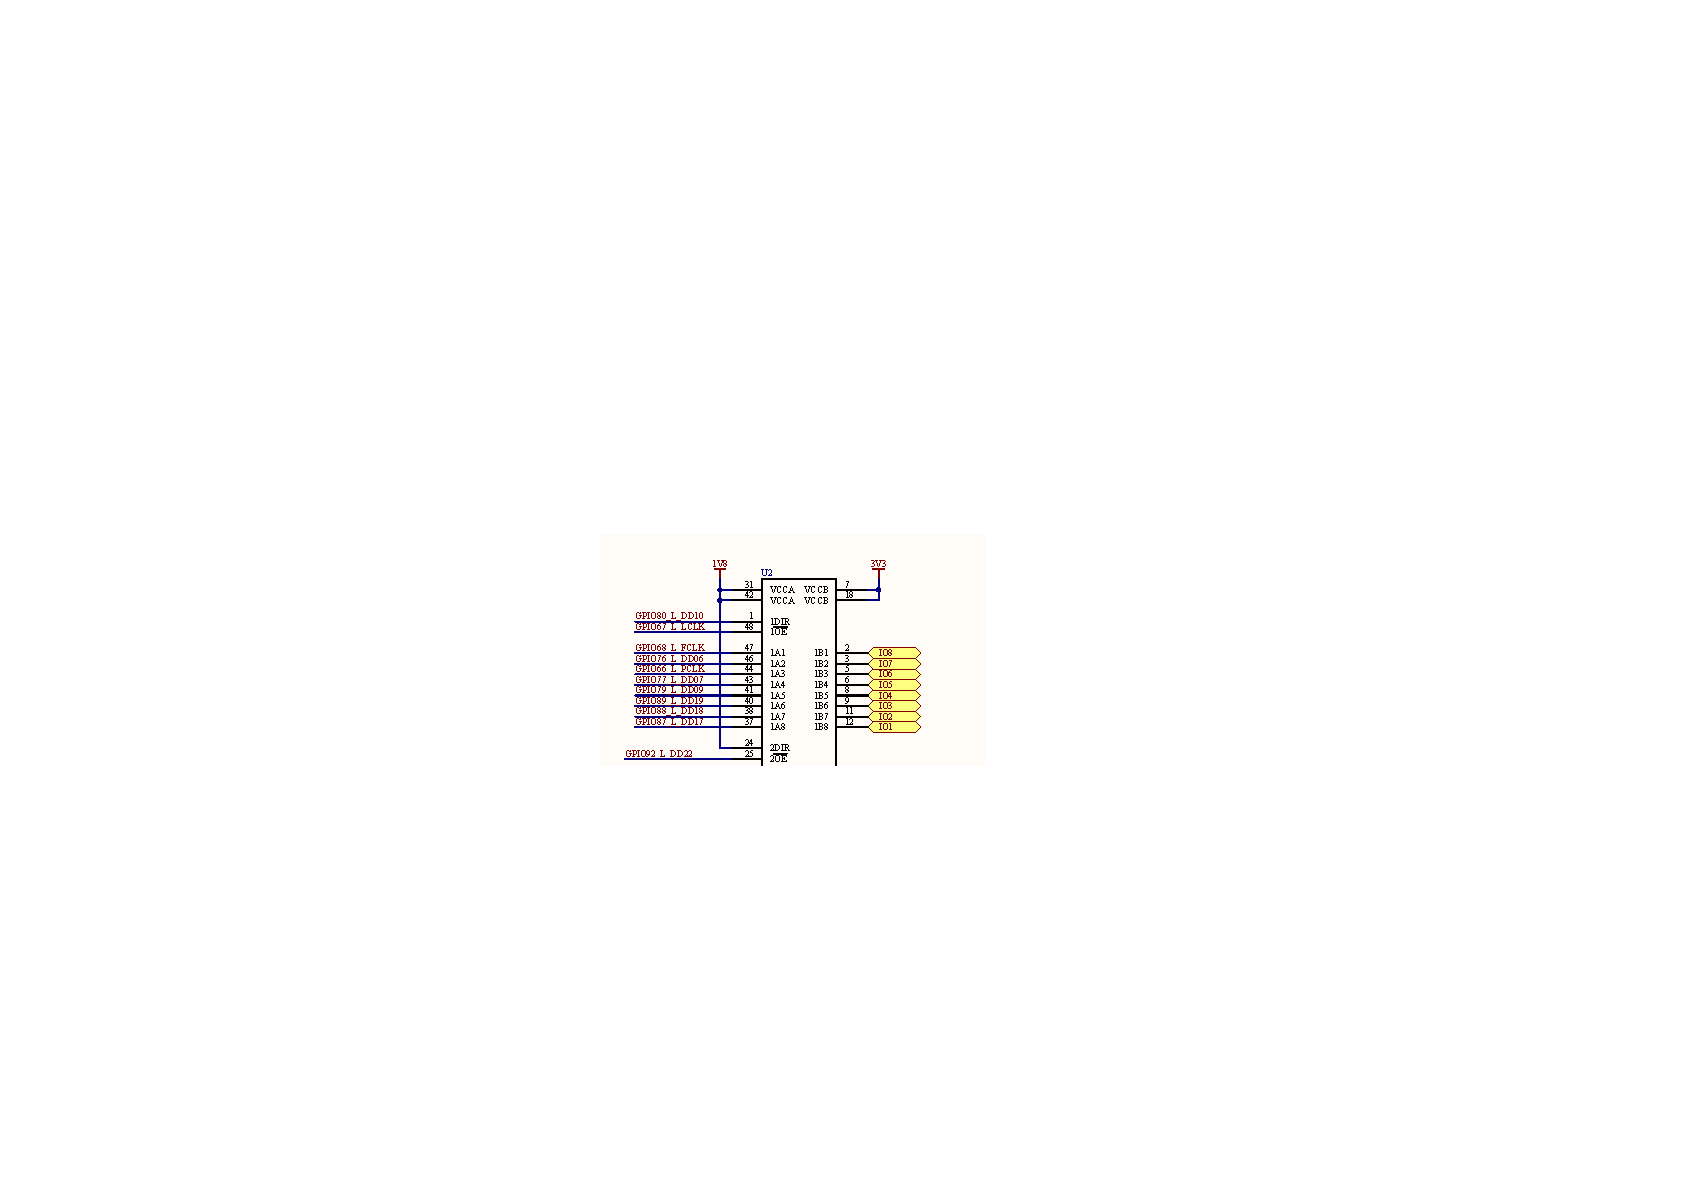
\includegraphics[width=15cm]{images/schematics-led.pdf}
\end{center}
\caption{Excerpt from the GumstixNXT schematics, level-shifter controlling LEDs}
\label{fig:led-levelshifter}
\end{figure}

To understand how to control the LEDs, we must consult the GumstixNXT
schematics (currently available under Blackboard).  The LEDs are
connected to a set of GPIO pins connected to the CPU via a
bidirectional level shifter, named ``U2'' on page 12 of the revision
1.0 schematics.  An excerpt of the relevant part of the diagram is
shown in Figure \ref{fig:led-levelshifter}, the LEDs are connected on
IO1\ldots IO9.

To output on the GPIOs connected to the level shifter, GPIO80
(direction) must be set to 1 (meaning output), GPIO 67 (output enable)
must be set to 0 (it is inverted, this means that it is activated),
and then GPIO68 (and a number of other GPIOs) can be used to toggle
the LED state of the LEDs (writing a zero to the GPIO sets it high,
turning on the LED).

To be able to use these GPIOs, the corresponding CPU pins must be
configured for GPIO usage.  The pins are multiplexed to many different
functionalities (modes), the mode must be set correctly on each of the
pins that we need to enable GPIO.  To find out what pins need to be
configured and how they must be configured, we need to consult the
datasheet for the CPU ``OMAP35x Applications Processor Technical
Reference Manual'' (available on Blackboard).  For example, to find
out how to enable GPIO67, we turn to page 772 which contains a part of
``Table 7-4. Core Control Module Pad Configuration Register Fields''
where we can see that GPIO67 is available on
``CONTROL\_PADCONF\_DSS\_PCLK[31:16]'' which is configured to
``dss\_hsync'' in Mode 0 must be configured to Mode 4 to enable
``gpio\_67''.

Following the ``Gumstix U-Boot development'' guide on jumpnowtek.com, we
change the pin multiplexing by modifying the overo.h file, e.g., the
line:
%
\begin{verbatim}
	MUX_VAL(CP(DSS_HSYNC),		(IDIS | PTD | DIS | M0)) /*DSS_HSYNC*/\
\end{verbatim}
%
is changed to
%
\begin{verbatim}
	MUX_VAL(CP(DSS_HSYNC),		(IEN  | PTU | DIS | M4)) /*GPIO_67*/\
\end{verbatim}
%
Since GPIO67 is accessed using register CONTROL\_\ldots\_HSYNC in mode
4.  All details of how to do this are described on jumpnowtek.com, the
recommended process is to modify the file, build a patch, add this
patch to the recipe, and rebuild.  (Note: the description on the web
page contains a few minor errors in the paths.)  The same changes must
be made for all of the GPIO pins that are needed (reading the
schematics in Figure \ref{fig:led-levelshifter}, these are GPIOs 80,
67, 68, 76, 66, 77, 79, 89, 88, and 87).

After rebuilding and redeploying, the appropriate ports are in GPIO
and can be used for blinking the LEDs, for example by directly
accessing the GPIO pins as described next.

\subsection{Direct hardware access using GPIO}

The kernel GPIO interface can be accessed directly from the shell:
%
\begin{verbatim}
root@overo:/root# cd /sys/class/gpio
root@overo:/sys/class/gpio# echo 80 > export
root@overo:/sys/class/gpio# echo 67 > export
root@overo:/sys/class/gpio# echo 68 > export
root@overo:/sys/class/gpio# echo out > gpio80/direction 
root@overo:/sys/class/gpio# echo out > gpio67/direction 
root@overo:/sys/class/gpio# echo out > gpio68/direction 
root@overo:/sys/class/gpio# echo 1 > gpio80/value 
root@overo:/sys/class/gpio# echo 0 > gpio67/value 
\end{verbatim}
%
These lines first export the appropriate GPIO pins (making the
accessible through /sys/class/gpio), set their direction to out, and
set GPIO80 and GPIO67 to the appropriate values.  Depending on how
else your environment is set up, one or more of the LEDs should now
light up.  

To blink an LED using GPIO68, use e.g.
\begin{verbatim}
  echo 0 > /sys/class/gpio/gpio68/value
\end{verbatim}
To turn it off, and to turn it back on again:
\begin{verbatim}
  echo 1 > /sys/class/gpio/gpio68/value
\end{verbatim}
Next step is to make a blinking LED program, which for example can be
done by creating the following script:
\begin{verbatim}
#!/bin/sh
for i in 0 1 2 3 4 5 6 7 8 9
do
  echo "Blink cycle $i"
  echo 0 > /sys/class/gpio/gpio68/value
  sleep 1
  echo 1 > /sys/class/gpio/gpio68/value
  sleep 1
done
\end{verbatim}
%
If you do not have a text editor, you can use 
\begin{verbatim}
cat > /root/blink.sh
  (...type the script, end with an empty line, press control-D...)
chmod 755 /root/blink.sh
\end{verbatim}
After which running /root/blink.sh will blink the LED 10 times.

\subsection{Adding utilities and helper scripts}

Next time you format the flash card and deploy the system the helper
scripts you just create will be removed.  It would be useful to have
an easy way of putting these onto the system, as you are working.  In
addition, using ``cat'' as a text editor obviously will not get you
very far if you need to edit something directly on the board.

We provide a Makefile for automating the task for formatting the SD
card, deploying the system, and easily adding extra files.  It is
available in the ``src/home'' directory\footnote{Using the current
  repository organization, the will probably change.}  The makefile
provides targets for format, building kernel modules (see later),
exporting all files stored in the ``export'' subdirectory, and
deploying everything to the SD card.

The default build includes the ``vi'' text editor.  If this is not
your cup of tea, there are numerous alternatives, such as the ``nano''
text editor that has fairly user-friendly keybindings.  To add this
editor to your image, edit ``myimage.bb'' (from above) adding the line
%
\begin{verbatim}
nano \
\end{verbatim}
%
to the ``IMAGE\_INSTALL'' variable.  Rebuilding will then download,
compile and include the nano editor, which will be available after
redeployment to the SD card.

%\section{Kernel Module Development}

%\subsection{LEDDEV 1-bit kernel module driver}

%\subsection{LEDDEV 8-bit kernel module driver}

%\subsection{Preliminary motor driver}

\newpage
\appendix

\section{Common error messages}

\subsection{Error messages during boot}

\begin{verbatim}
end_request: I/O error, dev mtdblock0, sector...
\end{verbatim}
This message can be ignored, it apparently has to do with a slight
incompatibility between the way the boot partition has been created and
what Linux expects.\footnote{Google search for the error message, see
  for example
  \url{http://old.nabble.com/What-is-mtdblock0-on-the-overo-earth-linux-omap3-2.6.29-build-td23179672.html}.}
Warning: apparently some people on the internet have rendered their
device incapable of booting by trying to fix this problem, so be
careful.

\section{LEDDEV 1-bit kernel module device driver}

\begin{verbatim}
/*

A gumstixtorms LED driver using GPIO, loosely based on irqlat by Scott
Ellis

*/

#include <linux/init.h>
#include <linux/module.h>
#include <linux/fs.h>
#include <linux/cdev.h>
#include <asm/uaccess.h>
#include <linux/string.h>
#include <linux/kernel.h>
#include <linux/device.h>
#include <mach/gpio.h>
#include <linux/interrupt.h>
#include <linux/workqueue.h>


#define GPIO_OE 80
#define GPIO_DIR 67

#define GPIO_BIT0 68

#define BIT_ON 0
#define BIT_OFF 1

struct leddev_dev {
  dev_t devt;
  struct cdev cdev;
  struct class *class;
  int value;
};

static struct leddev_dev leddev_dev;

/* Reset hardware settings and driver state */
static void leddev_reset(void)
{
  gpio_set_value(GPIO_OE, 1);
  gpio_set_value(GPIO_DIR, 0);
  gpio_set_value(GPIO_BIT0, BIT_OFF);
  leddev_dev.value = 0;
}

static ssize_t leddev_write(struct file *filp, const char __user *buff, size_t count, loff_t *f_pos)
{
  char cmd[4];
  ssize_t status = 1;
  int value;

  if (copy_from_user(cmd, buff, 1)) {
    printk(KERN_ALERT "Error copy_from_user\n");
    status = -EFAULT;
    goto leddev_write_done;
  }

  /*
    Nothing fancy, '1' means set the bit, '0' means unset, '-' means invert
  */
  if (cmd[0] == '1')
    leddev_dev.value = 1;
  else if (cmd[0] == '0')
    leddev_dev.value = 0;
  else if (cmd[0] == '-')
    leddev_dev.value = ~leddev_dev.value;

  value = leddev_dev.value;
  if(value&1)
    gpio_set_value(GPIO_BIT0, BIT_ON);
  else
    gpio_set_value(GPIO_BIT0, BIT_OFF);

 leddev_write_done:

  return status;
}

static const struct file_operations leddev_fops = {
  .owner = THIS_MODULE,
  .write = leddev_write,
};

static int __init leddev_init_cdev(void)
{
  int error;

  leddev_dev.devt = MKDEV(0, 0);

  error = alloc_chrdev_region(&leddev_dev.devt, 0, 1, "leddev");
  if (error < 0) {
    printk(KERN_ALERT
	   "alloc_chrdev_region() failed: error = %d \n",
	   error);

    return -1;
  }

  cdev_init(&leddev_dev.cdev, &leddev_fops);
  leddev_dev.cdev.owner = THIS_MODULE;

  error = cdev_add(&leddev_dev.cdev, leddev_dev.devt, 1);
  if (error) {
    printk(KERN_ALERT "cdev_add() failed: error = %d\n", error);
    unregister_chrdev_region(leddev_dev.devt, 1);
    return -1;
  }

  return 0;
}

static int __init leddev_init_class(void)
{
  leddev_dev.class = class_create(THIS_MODULE, "leddev");

  if (!leddev_dev.class) {
    printk(KERN_ALERT "class_create(leddev) failed\n");
    return -1;
  }

  if (!device_create(leddev_dev.class, NULL, leddev_dev.devt, NULL, "leddev")) {
    class_destroy(leddev_dev.class);
    return -1;
  }

  return 0;
}

static int __init leddev_init_pins(void)
{
  if (gpio_request(GPIO_OE, "OutputEnable")) {
    printk(KERN_ALERT "gpio_request failed\n");
    goto init_pins_fail_1;
  }

  if (gpio_direction_output(GPIO_OE, 0)) {
    printk(KERN_ALERT "gpio_direction_output GPIO_OE failed\n");
    goto init_pins_fail_2;
  }

  if (gpio_request(GPIO_DIR, "Direction")) {
    printk(KERN_ALERT "gpio_request(2) failed\n");
    goto init_pins_fail_2;
  }

  if (gpio_direction_output(GPIO_DIR, 0)) {
    printk(KERN_ALERT "gpio_direction_output GPIO_DIR failed\n");
    goto init_pins_fail_3;
  }

  if (gpio_request(GPIO_BIT0, "Bit0")) {
    printk(KERN_ALERT "gpio_request(3) failed\n");
    goto init_pins_fail_3;
  }

  if (gpio_direction_output(GPIO_BIT0, 0)) {
    printk(KERN_ALERT "gpio_direction_output GPIO_BIT0 failed\n");
    goto init_pins_fail_4;
  }

  return 0;

 init_pins_fail_4:
  gpio_free(GPIO_BIT0);

 init_pins_fail_3:
  gpio_free(GPIO_DIR);

 init_pins_fail_2:
  gpio_free(GPIO_OE);

 init_pins_fail_1:

  return -1;
}

static int __init leddev_init(void)
{
  memset(&leddev_dev, 0, sizeof(leddev_dev));

  if (leddev_init_cdev())
    goto init_fail_1;

  if (leddev_init_class())
    goto init_fail_2;

  if (leddev_init_pins() < 0)
    goto init_fail_3;

  leddev_reset();

  return 0;

 init_fail_3:
  device_destroy(leddev_dev.class, leddev_dev.devt);
  class_destroy(leddev_dev.class);

 init_fail_2:
  cdev_del(&leddev_dev.cdev);
  unregister_chrdev_region(leddev_dev.devt, 1);

 init_fail_1:

  return -1;
}
module_init(leddev_init);

static void __exit leddev_exit(void)
{
  gpio_free(GPIO_OE);
  gpio_free(GPIO_DIR);
  gpio_free(GPIO_BIT0);

  device_destroy(leddev_dev.class, leddev_dev.devt);
  class_destroy(leddev_dev.class);

  cdev_del(&leddev_dev.cdev);
  unregister_chrdev_region(leddev_dev.devt, 1);
}
module_exit(leddev_exit);

MODULE_AUTHOR("Ulrik Pagh Schultz");
MODULE_DESCRIPTION("A module for controlling gumstixstorms LEDs");
MODULE_LICENSE("Dual BSD/GPL");
MODULE_VERSION("0.1");
\end{verbatim}

\section{Quick guide to installing Ubuntu}
\label{app:getting-linux}

This guide assumes you are using Ubuntu 10.04 LTS (although 10.10 has
also been shown to work).  To get Ubuntu 10.04 LTS running on your
computer, there are basically three installation options:
%
\begin{enumerate}
\item Repartitioning your harddisk to make room for a Linux
  installation on a separate partition.
\item Installing Linux to an external media such as a USB harddrive.
\item Installing Linux using the Wubi installer, which installs Linux
  in a file on your Windows partition.
\end{enumerate}
%
If you know what you are doing, the first option gives you the best
performance, whereas the third option is both easy and quick and gives
fairly good performance.  The second option has not been tested and is
likely to not give stellar performance for the long-running
OpenEmbedded build process, it might work but we have not tested it.
The third option is recommended for beginners: it requires to have
enough free space on your harddrive, but then Linux is installed
transparently and can be selected when you reboot your machine.

The internet contains extensive information on these options.  Go to
www.ubuntu.com to read about Ubuntu, and search for ``Wubi'' on the
www.ubuntu.com website to learn more about it.  The OpenEmbedded
environment recommends having at least 60Gb of space on your
installation, but for the options we are using for our system it seems
to work with less: 40Gb of space seems to work.

\section{Notes on using a virtualized host for development}
\label{app:virtualized}

You can use a virtualized host for your development, but it puts
certain requirements on the operating system running on the physical
machine.  Compiling open embedded can be done in any host with
appropriate resources, e.g.\ 2Gb of RAM and a 40Gb filesystem works
with Ubuntu (although 60Gb is apparently recommended).  The hard part is interacting with the SD card, which
requires the ability to partition (MBR scheme) and create filesystems
(FAT and EXT3).  We have tried two different options: attaching the
card reader directly to the virtualized host, and using Mac OS to
interact with the SD card.

\subsection{Attaching card reader to virtualized host}

This approach has been verified to work with VMWare 3.x and Mac OS,
has been abandoned for Windows 7 due to technical complications, and
seems more likely to work with Windows XP (but this is untested).  The
idea is to simply attach the SD card reader directly to the
virtualized host as a USB device, this allows the virtualized host
full control over low-level access to the SD card (but apparently this
does not work very well under Windows 7).  Note that many
internal SD card readers are also attached via USB.  Using this
approach the SD card becomes directly accessible as a device under
\out{/dev}, and can be used as described earlier in this document..

\subsection{Using Mac OS to interact with the SD card}

This approach is apparently very close to working, but has not been
shown to be completely functional.  The prerequisites are that you are
using macports with the packages e2fsprogs, ext2fuse, and macfuse
installed.

Partitioning can be done using fdisk; the functionality is equivalent
to Linux fdisk but the interface is very simplistic.  Nevertheless,
using the -d and -r options one can save and restore partition
schemes from an SD card.  So using fdisk with -d one can save the
table from one card, and then write it to another card of the same
size using the -r option.

Formatting is simple, the required utilities are available either by
default or using the aforementioned macports packages:
\begin{verbatim}
sudo newfs_msdos -F 32 /dev/disk2s1
sudo mkfs.ext3 /dev/disk2s2
\end{verbatim}

Mounting the card partitions is however not so easy.  The FAT
partition mounts automatically and can be mounted manually using e.g.:
\begin{verbatim}
sudo mount -t msdos /dev/disk2s1 mnt/card
\end{verbatim}
The EXT3 partition is however not easily mounted.  Using FUSE one can
mount EXT2/3 partitions, as follows:
\begin{verbatim}
sudo ext2fuse /dev/disk2s2 mnt/card -o force,allow_other &
\end{verbatim}
This almost works except that apparently it cannot create /dev special
files and hard links, both of which is required for creating the basic
Linux file system.  If this problem could be resolved then the
approach would work.  (Alternatively the EXT3 filesystem could be
created from within Linux as an image that was then copied to the SD
card using the dd command, this works but is too slow for e.g.\ a 4 Gb
card since it requires to transfer all the data for the entire
partition.)

\end{document}
